\begin{abstract}
Tool-calling agents are built against a tool schema. The schema then versions: fields get renamed, enums get tightened, optional arguments become required, types change, defaults change. We measure what happens when the schema changes and the agent is not told. We freeze SchemaDrift-120, a testbed of 30 tools and 120 programmatically checkable tasks, and apply five deterministic drift classes as minimal pairs, so every drifted schema differs from its original by exactly one change. Four model families act as agents (Gemini 3.6 Flash, Gemini 3.1 Pro, GPT-5.6-luna, Qwen2.5-7B) across 4,800 episodes. First, drift is severe: task success falls from 87 to 99 percent at baseline to 11 to 38 percent when the executor silently enforces the new schema (all four paired drops $p < 5\times10^{-5}$). Second, whether the failure is visible depends jointly on the drift class and the API's tolerance policy: default changes never raise an error under any validator, and a lenient executor converts 67 to 100 percent of rename and type drift into calls that are accepted with wrong semantics. A hand audit of 24 such calls confirms all 24, including an \$80 payment executed as EUR 80 and a two day access grant executed as four months. Third, a machine-readable schema diff in context, 13.7 percent of the schema's token size, recovers 96 to 98 percent of the lost success on both Gemini models and outperforms re-injecting the full new schema (82 to 83 percent), because the diff carries the old contract, including deleted defaults, which the new schema alone does not. Fourth, the same diff recovers nothing on Qwen2.5-7B (0.06) and nothing on GPT-5.6-luna (point estimate $-0.06$): transcripts show both models keep emitting old-schema calls with the diff in context. Fifth, exposure itself is a property of calling style: GPT-5.6-luna fills every optional parameter explicitly and is therefore mechanically immune to newly-required and default-change drift (96 percent survival versus 25 to 31 percent for the Gemini models), while remaining fully exposed to renames, enum changes, and type changes. Schema drift is a correctness hazard that validators and retry loops structurally miss, and the cheapest repair, serving a diff, only works for models that read it.
\end{abstract}

\section{Introduction}

An agent that calls tools is executing someone else's interface. The interface is described by a schema: a function name, typed parameters, enums, required flags, and documented defaults. The agent's prompt carries a copy of that schema. The service behind the tool enforces its own copy. These two copies are assumed to be the same one.

In deployment they drift apart. Services version their APIs on their own schedule. A parameter is renamed, an enum value is retired, an optional field becomes mandatory, an integer becomes a formatted string, a default flips. The Model Context Protocol (MCP) ecosystem, where agents load tool declarations from independently maintained servers, makes this an everyday event rather than a rare migration \citep{mcpfaults}. Recent benchmarks have established the headline consequence: agents degrade when tool interfaces evolve \citep{mcpevol, toolbenchx, proevolve}. What those benchmarks do not tell us is the part a practitioner most needs: when a drifted call fails, does anyone find out, and what is the cheapest thing that fixes it?

This paper answers both questions with a controlled instrument. We freeze a testbed before applying any drift: 30 tools across ten domains and 120 tasks whose correct calls are checkable by a script, with two phrasings per task. We then apply five deterministic drift classes as minimal pairs. Each drifted schema differs from its original by exactly one change: a parameter rename, an enum tightening, an optional parameter promoted to required, an integer changed to a formatted string, or a changed default. Because the transforms are deterministic and single-edit, every failure is attributable to a known cause. This is the difference between our instrument and the model-generated compound mutations of prior evolution benchmarks \citep{mcpevol, toolbenchx}, which establish that degradation happens but cannot cleanly attribute it.

A local executor enforces the active schema and returns realistic error strings, or accepts the call. It runs under two tolerance profiles, because real APIs genuinely differ: a strict profile that rejects unknown parameters and type mismatches, and a lenient profile that silently drops unknown parameters and coerces types, which is common gateway behavior. Every drifted call lands in a three-way ledger: an error was surfaced, the call was accepted and correct, or the call was accepted with wrong semantics. The last cell is the one that should worry practitioners, and we hand-audit a sample of it.

On top of the drifted condition we compare three recovery levers, holding everything else fixed: (i) a structured, machine-readable diff of the schema change added to context, (ii) the full new schema replacing the stale one, and (iii) one retry with the raw executor error string. The diff is the cheap lever: it averages 28 tokens against 206 for a full schema declaration, 13.7 percent of the size, and in a large tool catalog it is the only artifact whose cost scales with the change rather than with the catalog.

Our contributions:
\begin{enumerate}
\item \textbf{SchemaDrift-120}, a frozen drift instrument: five deterministic minimal-pair drift classes over 30 tools and 120 checkable tasks, 48 task-drift pairs per class, with a dual-profile executor and a per-call outcome ledger (\S\ref{sec:method}).
\item \textbf{A drift-class by tolerance-policy map of silent failure} (\S\ref{sec:results-drop}, \S\ref{sec:results-ledger}): default changes surface no error under any validator; a lenient executor converts 67 to 100 percent of rename and type drift into accepted calls with wrong semantics; enum and newly-required drift reliably surface errors. All 24 audited wrong-semantics calls are confirmed wrong, several with money or access-control consequences.
\item \textbf{A controlled three-way recovery comparison} (\S\ref{sec:results-levers}): the diff recovers 0.96 to 0.98 of the lost success on Gemini models, beating full-schema re-injection (0.82 to 0.83) because the diff carries the old contract, and recovers approximately nothing on GPT-5.6-luna and Qwen2.5-7B, which ignore it. The raw-error retry recovers at most 0.39 anywhere and exactly nothing on the drift class that never errors.
\item \textbf{Calling style as a mechanical exposure axis} (\S\ref{sec:results-style}): the share of optional parameters a model fills explicitly (0.45 to 1.00 across our families) predicts its survival on newly-required and default-change drift (0.25 to 0.96), a model-level property no prior drift work separates.
\end{enumerate}

\section{What was known and what is new}
\label{sec:known}

The premise that agents degrade under tool evolution is not ours. We list the closest prior work and the specific claim of ours that each does not cover.

\begin{table}[h]
\small
\centering
\begin{tabular}{p{4.6cm}p{8.6cm}}
\toprule
\textbf{Closest neighbor} & \textbf{What it established / what it does not cover} \\
\midrule
MCPEvol-Bench \citep{mcpevol} & 12 LLMs degrade 13 to 14 percent under LLM-simulated, backward-compatible MCP server evolution. No breaking minimal-pair transforms, no silent-failure accounting, no recovery lever that informs the agent of the change. \\
ToolBench-X \citep{toolbenchx} & Specification drift as one of five injected hazards; post-failure natural-language hints recover 60 to 80 percent. Drift instances are LLM-generated rewrites; hints are prose after task failure; its executor silently mutates payloads without measuring acceptance with wrong semantics. \\
ToolMisuseBench \citep{toolmisuse} & Deterministic fault injection including call-level drift, with rule-based schema repair. Mutates the emitted call, not the schema the agent believes; no LLM prompting levers; no wrong-semantics cell. \\
SilentProbe \citep{silentprobe} & Silent (HTTP 200) failures of live production API tools; models detect 12 percent. Failures come from schema-prose gaps in static APIs, not from induced, attributable drift. \\
Diff-based code migration \citep{whatadiff, deprepair, recode} & Diffs in context improve LLM code migration. Different task and failure surface; not a tool-calling agent at inference time, and no comparison against schema re-injection or error retry. \\
Silent-failure studies \citep{falsesuccess, errnarratives, reflecterr} & False success is common in agents generally. Not attributed to schema drift, and not conditioned on a known drift class. \\
\bottomrule
\end{tabular}
\caption{Novelty delineation. Full related work in \S\ref{sec:related}.}
\label{tab:delineation}
\end{table}

What is new here: the deterministic minimal-pair drift taxonomy with per-class attribution, the error-surfaced versus accepted-wrong ledger conditional on a known induced drift class and executor policy, the controlled diff versus full-schema versus retry comparison, and the calling-style exposure axis.

\textbf{Significance.} Who is affected: anyone shipping agents against MCP servers or OpenAPI backends that version independently of the agent's prompt. What changes: if a serving stack adds one machine-readable diff artifact to version bumps, the drift problem becomes nearly free to fix for model families that apply diffs, at about one seventh the token cost of re-serving schemas. And because default-change drift surfaces no error anywhere, monitoring built on error rates will report a healthy system while payments go out in the wrong currency; the accepted-wrong cell needs its own monitoring.

\section{Method}
\label{sec:method}

\begin{figure}[t]
\centering
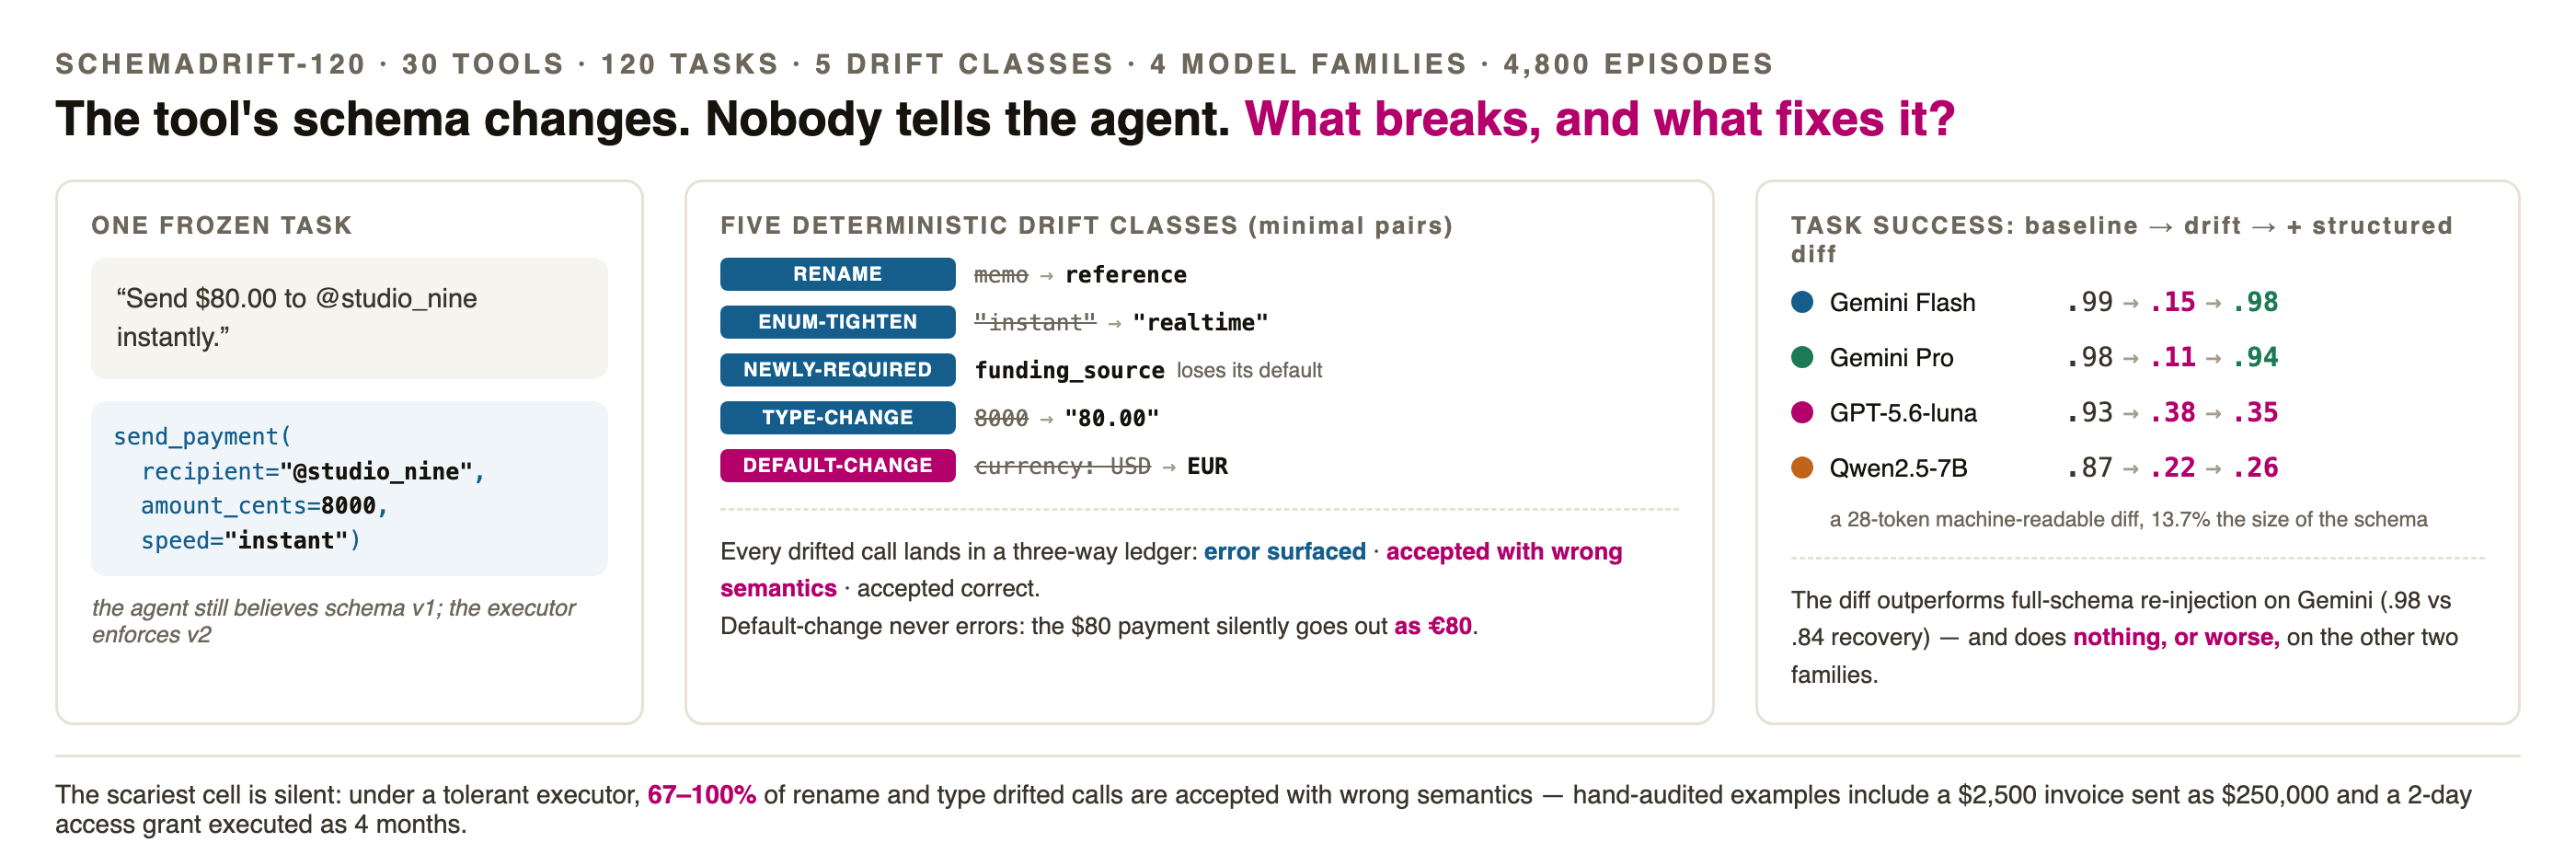
\includegraphics[width=\textwidth]{assets/fig1_teaser.png}
\caption{Study design and headline numbers. One frozen task, five deterministic drift classes applied to the tool schema as minimal pairs, a dual-profile executor with a three-way outcome ledger, and the measured effect of a 28-token schema diff on four model families.}
\label{fig:teaser}
\end{figure}

\textbf{Testbed.} SchemaDrift-120 contains 30 tools, three in each of ten domains (calendar, payments, filesystem, CRM, messaging, web search, e-commerce, travel, HR, analytics). Each tool is a JSON-schema function declaration with 3 to 7 parameters and carries, by construction, at least one enum parameter, one optional parameter with a documented default, one integer parameter, and one renameable optional parameter, so every drift class applies to every tool. There are 120 tasks, four per tool: 90 single-step and 30 two-step (at most three agent turns, with tool results fed back). Each task is a natural-language request plus frozen ground-truth calls. Correctness is checked by a script: canonicalized argument matching (sorted keys, numeric equivalence, ISO-8601 normalization, case-insensitive free strings) with active-schema defaults filled before comparison. Each task has two phrasings; phrasing one is primary and phrasing two feeds a robustness battery. The testbed was frozen, with a recorded hash, before any drifted episode ran. One amendment happened during a pre-drift baseline calibration pass and is documented in Appendix~\ref{app:freeze}.

\textbf{Drift classes.} Five deterministic transforms, each applied alone (Table~\ref{tab:classes}). Assignment is balanced: every task carries two assigned classes that target parameters its ground truth actually uses, giving 240 task-drift pairs, 48 per class; a primary subset of 120 pairs (24 per class) is what every family runs, and the cheaper families run all 240.

\begin{table}[h]
\small
\centering
\begin{tabular}{llll}
\toprule
Class & Transform & Example & Ground truth under v2 \\
\midrule
\textsc{rename} & optional param renamed & \texttt{memo} $\to$ \texttt{reference} & key renamed \\
\textsc{enum-tighten} & used enum value replaced & \texttt{instant} $\to$ \texttt{realtime} & new value \\
\textsc{newly-required} & optional param loses default & \texttt{funding\_source} required & old default, explicit \\
\textsc{type-change} & int $\to$ formatted string & \texttt{8000} $\to$ \texttt{"80.00"} & converted value \\
\textsc{default-change} & documented default changes & currency \texttt{USD} $\to$ \texttt{EUR} & old default, explicit \\
\bottomrule
\end{tabular}
\caption{The five drift classes. Each drifted schema differs from v1 by exactly this one change.}
\label{tab:classes}
\end{table}

\textbf{Executor and ledger.} A local mock executor validates each call against the active schema and returns either a realistic error string (modeled on pydantic and Stripe error formats; verbatim in Appendix~\ref{app:prompts}) or acceptance, after which omitted optional parameters take the active schema's defaults. Two tolerance profiles are both measured, because which drifts \emph{can} surface an error is partly the API's choice, not the model's: \emph{strict} rejects unknown parameters, missing required parameters, enum violations, and type mismatches; \emph{lenient} silently drops unknown parameters and coerces representable types, and still rejects missing required parameters and enum violations. Every drifted call is classified as \textsc{error-surfaced}, \textsc{accepted-correct}, or \textsc{accepted-wrong} (accepted with no error while its executed semantics, after default filling, differ from the user's intent).

\textbf{Conditions.} Per task-drift pair: (A) the agent sees v1 and the executor enforces v1, the baseline; (B) the agent sees v1 while the executor enforces v2, under both profiles, the silent-drift core; (C) as B strict, plus a structured JSON diff of the change in the system prompt; (D) the agent sees the full v2 schema; (E) as B strict, with the raw error string returned and one retry. The diff format is a per-field change record with old and new values; verbatim in Appendix~\ref{app:prompts}.

\textbf{Models and protocol.} Gemini 3.6 Flash and Gemini 3.1 Pro through the native API (temperature 0, thinking minimal and low respectively), GPT-5.6-luna through an OpenAI-compatible gateway (temperature 0), and Qwen2.5-7B-Instruct on vLLM with the hermes tool template (greedy) on a single A10G. One episode per record, randomized order, resume-safe. Flash and Qwen run the full grid (240 pairs, both profiles, plus batteries); Pro and GPT-5.6-luna run the primary 120 pairs. Total: 4,800 episodes. The full study cost under 8 US dollars of metered API spend plus 1.7 GPU hours.

\textbf{Analysis.} The unit is the within-pair paired difference: bootstrap 95 percent confidence intervals (10,000 resamples), two-sided sign-flip permutation tests (20,000 permutations), and paired $d_z$. Recovery fraction for lever $X$ is $(\mathrm{succ}(X) - \mathrm{succ}(B))/(\mathrm{succ}(A) - \mathrm{succ}(B))$ with bootstrap intervals over pairs. Drift-class by condition interactions are tested directly by permuting class labels over pairs. Benjamini-Hochberg correction runs over all 112 reported tests; 74 survive at the effective threshold $p \le 0.0316$, and only survivors are bolded in tables. Every number in this paper is produced by one scripted analysis reading the raw episode logs.

\section{Results}

\subsection{Drift removes 55 to 87 points of task success}
\label{sec:results-drop}

Table~\ref{tab:main} and Figure~\ref{fig:conditions} (left) give the study in one view. Baselines are high (0.87 to 0.99), so the tasks are within every family's competence. Silent drift under the strict executor removes most of it: the paired drop is $+0.84$ [0.79, 0.88] for Flash, $+0.87$ [0.80, 0.93] for Pro, $+0.55$ [0.46, 0.63] for GPT-5.6-luna, and $+0.65$ [0.58, 0.70] for Qwen (all $p < 5\times10^{-5}$, $d_z$ 1.10 to 2.54). The lenient executor changes the failure mode, not the level (success 0.19 to 0.44).

\begin{table}[t]
\small
\centering
\begin{tabular}{lcccccc}
\toprule
 & \multicolumn{6}{c}{Task success} \\
\cmidrule(lr){2-7}
Model & A base & B strict & B lenient & C +diff & D +v2 schema & E +retry \\
\midrule
Gemini 3.6 Flash ($n{=}240$) & .992 & .154 & .204 & \textbf{.975} & \textbf{.838} & \textbf{.442} \\
Gemini 3.1 Pro ($n{=}120$) & .975 & .108 & .192 & \textbf{.942} & \textbf{.825} & \textbf{.342} \\
GPT-5.6-luna ($n{=}120$) & .933 & .383 & .442 & .350 & \textbf{.692} & .367 \\
Qwen2.5-7B ($n{=}240$) & .867 & .221 & .263 & .263 & \textbf{.646} & \textbf{.471} \\
\bottomrule
\end{tabular}
\caption{Task success by condition. $n$ is task-drift pairs; A is per task. Bold in columns C, D, E: the paired difference against B strict survives Benjamini-Hochberg over all 112 tests. Per-class tables in Appendix~\ref{app:tables}.}
\label{tab:main}
\end{table}

\begin{figure}[t]
\centering
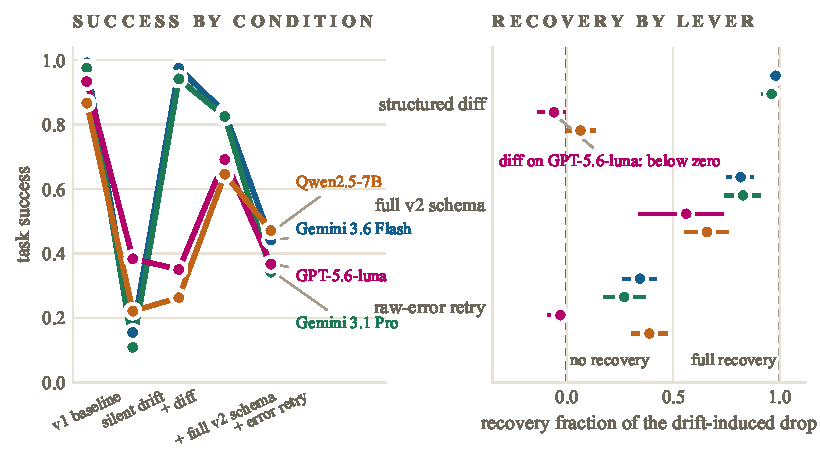
\includegraphics[width=\textwidth]{assets/fig2_conditions_recovery.pdf}
\caption{\textbf{Left:} success by condition for the four families. \textbf{Right:} recovery fraction of the drift-induced drop per lever, with bootstrap 95 percent intervals; right of the zero line means the lever recovered something. The diff (top row) splits the families: near-total recovery for both Gemini models, approximately zero for Qwen2.5-7B, and a negative point estimate for GPT-5.6-luna.}
\label{fig:conditions}
\end{figure}

\subsection{Whether drift is visible depends on the class and on the API's tolerance}
\label{sec:results-ledger}

Figure~\ref{fig:ledger} shows the outcome ledger for Flash (other families in Appendix~\ref{app:tables}). Under the strict executor, four classes surface errors on essentially every failed call: rename, enum-tighten, newly-required, and type-change (85 to 100 percent \textsc{error-surfaced}). \textsc{default-change} is the exception: it violates nothing a validator can check, so it never errors anywhere; 38 percent of Flash's default-change calls are \textsc{accepted-wrong} even under strict validation, and the remaining 62 percent survive only because the model happened to pass the cued value explicitly.

The lenient profile rewrites the map. Renamed parameters are silently dropped, so 100 percent of Flash's rename-drift calls become \textsc{accepted-wrong}: the call succeeds and the renamed field's content is simply gone, replaced by the new default. Type drift is coerced: 75 percent accepted with the wrong scale (an integer 8000 becomes the string "8000" where "80.00" was meant). The same tolerance policies that make APIs pleasant to integrate against convert two drift classes from loud to silent.

This has a direct consequence for the retry lever: \emph{a retry loop can only fix what errors}. Per-class recovery for E on Flash is 0.98 on newly-required (the error names the missing parameter and the old default is documented in the stale schema) and 0.53 on enum-tighten (the error lists the allowed values), but 0.00 on rename, 0.04 on type-change (the error names the parameter but not the old-to-new mapping), and $-0.06$ on default-change, where there is no error to retry from.

\begin{figure}[t]
\centering
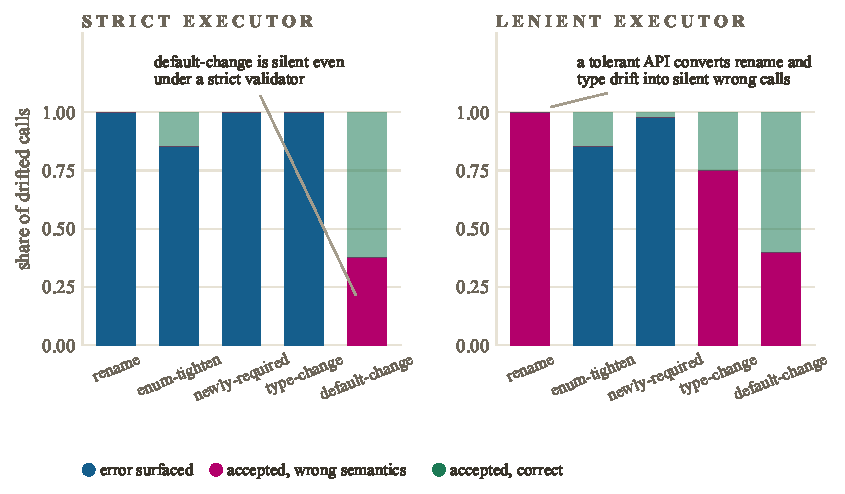
\includegraphics[width=\textwidth]{assets/fig3_ledger.pdf}
\caption{The outcome ledger for Gemini 3.6 Flash under silent drift, $n{=}48$ drifted calls per class. \textbf{Left:} strict executor. \textbf{Right:} lenient executor. Default-change never surfaces an error under either profile; the lenient profile converts rename and type drift into accepted calls with wrong semantics.}
\label{fig:ledger}
\end{figure}

\subsection{The diff lever: near-total recovery, but only for families that read it}
\label{sec:results-levers}

The right panel of Figure~\ref{fig:conditions} is the paper's central result. On the Gemini models the structured diff recovers 0.98 [0.95, 1.00] (Flash) and 0.96 [0.92, 0.99] (Pro) of the lost success, at a mean artifact size of 28 tokens against 206 for the full schema (13.7 percent). The diff beats full-schema re-injection (0.82 [0.76, 0.87] and 0.83 [0.75, 0.90]). The mechanism is visible in the per-class breakdown: on newly-required drift, D recovers only 0.40 on Flash while C recovers 1.00, because the new schema shows that the parameter is required but no longer contains the deleted default value; the diff carries the old contract, so the agent knows both that the field is now mandatory and what value preserves the old behavior. The same holds for default-change (C 0.89 versus D 0.83). A diff is not merely a compressed schema; it is strictly more informative about the past.

On the other two families the lever fails. Qwen2.5-7B: recovery 0.06 [0.01, 0.13], paired difference $+0.042$, $p = 0.064$, not significant after correction. GPT-5.6-luna: recovery point estimate $-0.06$ [$-0.13$, $-0.01$], paired difference $-0.033$, $p = 0.12$, also not significant after correction; what is established is the absence of recovery, with a negative point estimate. Transcripts show the failure is not subtle: under condition C both models keep emitting v1-style calls with the change log sitting in the system prompt, and on GPT-5.6-luna the note occasionally perturbs calls on pairs it would otherwise have survived. Full-schema re-injection, by contrast, transfers everywhere (0.56 to 0.83, all surviving correction). The drift-class by condition interaction is significant for every lever on the Gemini models and for D and E on Qwen ($p < 5\times10^{-4}$ by label permutation), confirming that lever effectiveness genuinely differs by class rather than only by level.

\subsection{Calling style is a mechanical exposure axis}
\label{sec:results-style}

Why does GPT-5.6-luna lose only 55 points where Pro loses 87? Not robustness in any adaptive sense. GPT-5.6-luna passes every optional parameter explicitly in its baseline calls (fill rate 1.00, against 0.45 for Flash, 0.46 for Pro, 0.71 for Qwen). A model that always writes \texttt{currency="USD"} itself cannot be hurt when the default changes, and cannot omit a parameter that just became required. Its survival on those two classes is 0.96, against 0.25 to 0.31 for the Gemini models; on the three classes that defensive filling cannot help (rename, enum, type), every family is equally destroyed (survival 0.00 to 0.05). Figure~\ref{fig:argstyle} plots the relationship across the four families. Exposure to two of the five drift classes is set by an argument-writing habit, before any reasoning about change happens.

\begin{figure}[t]
\centering
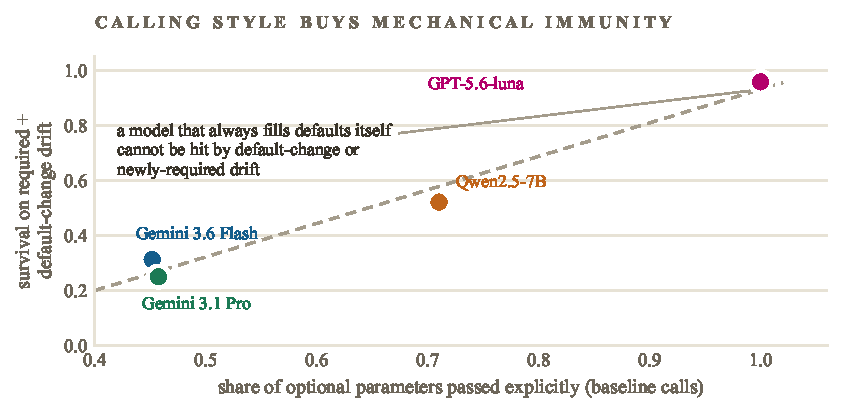
\includegraphics[width=\textwidth]{assets/fig4_argstyle.pdf}
\caption{Share of optional parameters filled explicitly at baseline (x) against survival on newly-required plus default-change drift under silent drift (y), one point per family. Defensive filling is mechanical immunity to exactly these two classes; it does nothing for rename, enum, or type drift.}
\label{fig:argstyle}
\end{figure}

\subsection{The accepted-wrong cell, audited}
\label{sec:results-audit}

Rates alone understate this cell, so we hand-verified a stratified sample of 24 \textsc{accepted-wrong} episodes across all four families and all five classes (audit file ships with the release). All 24 are confirmed: the call was accepted without any error and did something other than what the user asked. The concrete shapes: a payment of \$80.00 executed as EUR 80 after a currency default change; a \$375.50 invoice issued as \$37,550 and a \$2,500 invoice as \$250,000 after integer-cents to decimal-string type drift met lenient coercion; a two day access grant executed as a 2,880 hour grant; a Toronto job posting published as remote after a renamed location field was silently dropped; a customer never notified of a refund after a notification default flipped. Two of the 24 are low-stakes (a bookmark folder, a deal metadata field), and in two the wrong value was partly model-invented rather than purely mechanical; we label these in the audit file. Under the lenient executor these are exactly the calls a monitoring dashboard counts as successes.

\subsection{Batteries: noise, phrasing, and correction}
\label{sec:results-batteries}

Thirty stratified pairs were re-run five times each under silent drift: 13.3 percent of Flash pairs flip success at least once across five identical calls at temperature 0; Qwen under greedy decoding flips zero. The headline effects (55 to 87 point drops, 60 to 82 point lever gaps) are far outside this noise floor. Re-running baseline and drift conditions on the second phrasing of every task moves success by at most 4.2 points (all $p \ge 0.27$), so the results are not a property of one phrasing. Benjamini-Hochberg over all 112 reported tests retains 74 at an effective threshold of $p \le 0.0316$, including every effect named in the abstract; individual cells that fail correction are marked and should be read as unconfirmed.

\section{Limitations, narrated}
\label{sec:limitations}

The executor is a mock. Its two tolerance profiles bracket real API behavior rather than sample it; the ledger's per-class silent rates are therefore properties of drift class \emph{times policy}, which is the claim, but the mix of policies in production is not measured here. The silent-failure composition we report is partly a design consequence: we chose type conversions where naive coercion yields a valid but wrongly scaled value, because that is the dangerous case; conversions that fail coercion would surface errors instead.

Our pre-registered directions did not all survive. We recorded, before any data, the direction that newly-required arguments would cause the largest silent failure rate. The opposite is true: newly-required drift is the most reliably surfaced class, and default-change is the silent one. We noted at registration time that the executor mechanics might force exactly this reversal, and they did; we report it as a reversal. The token-cost direction (diff under 10 percent of schema size) also missed: the measured ratio is 13.7 percent.

The diff result is a capability statement about four checkpoints in September 2026, not a law. The negative results on GPT-5.6-luna and Qwen do not survive multiple-comparison correction as harms; they are absences of benefit. We did not test whether prompting harder (for example, an instruction to apply the change log step by step) unlocks diff-following on those families; that is one experiment away and would sharpen the deployment advice.

The testbed is synthetic and English-only, with 30 tools and single-edit drift. Real drift arrives in bundles, with changelogs of mixed quality, and on tool catalogs an order of magnitude larger, where the token argument for diffs gets stronger but the retrieval problem (which diff applies to this call) appears. Two-step tasks cap at three turns. One phrasing battery and a five-repeat noise floor bound but do not eliminate stochastic and phrasing variance. The 24-call audit covers the cell's variety, not its full population.

\section{Related work}
\label{sec:related}

\textbf{Tool evolution and drift.} MCPEvol-Bench \citep{mcpevol} and ProEvolve \citep{proevolve} establish degradation under evolving tool environments with LLM-driven mutations; ToolBench-X \citep{toolbenchx} injects specification drift among five hazards and shows prose hints help after failure; ToolMisuseBench \citep{toolmisuse} injects call-level drift deterministically with rule-based repair; ReliabilityBench \citep{reliabilitybench} and LayerRAG-Bench \citep{layerrag} include schema drift among stress faults; skill libraries decay as contracts change \citep{skilldrift}. None isolates single drift classes, none measures acceptance with wrong semantics, and none compares change-information levers.

\textbf{Robustness and static benchmarks.} The classic tool-use benchmarks evaluate static contracts \citep{toolllm, apibank, toolalpaca, teval, taubench, agentbench, toolemu, metatool, bfcl}. RoTBench \citep{rotbench} perturbs the schema the model is shown, adversarial noise on a static contract, whereas our drift is a believed-versus-enforced mismatch. StableToolBench \citep{stabletool} responds to real API instability by freezing it away, which is the strongest evidence the phenomenon matters. ToolRobustBench \citep{toolrobust} and ToolMaze \citep{toolmaze} perturb interfaces and runtime behavior at the tool level.

\textbf{Silent failure.} A 2026 wave documents false success in agents \citep{falsesuccess, errnarratives, reflecterr}; SilentProbe \citep{silentprobe} measures silent failure against live production APIs; an MCP audit finds error results rarely actionable \citep{mcpaction}. We add the attribution: which induced drift class, under which tolerance policy, produces silence.

\textbf{Recovery mechanisms.} Error-feedback repair and reflection are well studied \citep{reflexion, critic, structreflect, toolcritic, structfeedback, backfires, selfreflective, bench2robust, agentcheck}; constrained decoding guarantees validity against the schema the client believes, which under drift validates against the wrong contract \citep{tooldec}. Diff-conditioning exists in code migration \citep{whatadiff, deprepair, recode}; we test the same lever for tool-calling agents at inference time, against re-injection and retry.

\section{Conclusion}

We versioned tool schemas out from under four agent families with five single-edit drift classes and an executor whose tolerance policy we controlled. Drift removes 55 to 87 points of task success. Whether anyone finds out depends on the class and the policy: default changes are silent everywhere, and a lenient gateway turns renames and type changes into confidently wrong calls, of which all 24 audited examples were genuinely wrong, some expensively. A 28-token machine-readable diff repairs nearly everything for the two models that apply it, and beats re-serving the full schema because it carries the deleted past. The same artifact does nothing for the two models that ignore it, and a model's private habit of filling every optional argument decides, before any recovery lever runs, whether two of the five drift classes can touch it at all. The practitioner reading: version bumps should ship machine-readable diffs; error-rate monitoring does not cover default changes; and both the benefit of the diff and the exposure to drift are properties of the model family you deploy, so they belong in the evaluation you run before choosing it.

\subsubsection*{Reproducibility statement}
The frozen testbed (with its hash), all drift transforms, the executor, every runner, the raw episode logs, the scripted analysis producing every number in this paper, the audit sample with verdicts, and the spend log accompany this submission and will be released publicly. Total marginal compute: under 8 US dollars of metered API spend and 1.7 GPU hours on one A10G.

\subsubsection*{LLM usage statement}
Large language models are the subjects of this study (the four agent families under test) and served as engineering assistants for analysis code, figures, and manuscript editing. All experimental design choices, statistical decisions, interpretations, and claims are the authors'; every reported number was checked against the scripted analysis output before entering the text.
